\documentclass{article}
\usepackage{PRIMEarxiv}
\usepackage[utf8]{inputenc} % allow utf-8 input
\usepackage[T1]{fontenc}    % use 8-bit T1 fonts
\usepackage{palatino,eulervm}
\usepackage{hyperref}       % hyperlinks
\usepackage{url}            % simple URL typesetting
\usepackage{booktabs}       % professional-quality tables
\usepackage{amsfonts}       % blackboard math symbols
\usepackage{nicefrac}       % compact symbols for 1/2, etc.
\usepackage{microtype}      % microtypography
\usepackage{lipsum}
\usepackage{fancyhdr}       % header
\usepackage{graphicx}       % graphics
\graphicspath{{media/}}     % organize your images and other figures under media/ folder

\pagestyle{fancy}
\thispagestyle{empty}
\rhead{ \textit{ }} 
  
\title{Kalman Filters and Homography: Utilizing the Matrix $A$}

\author{
  Burak Bayramlı \\
  İstanbul, Turkey\\
  \texttt{burakbayramli.github.io} 
}


\begin{document}
\maketitle

\begin{abstract}
Many problems in Computer Vision can be reduced to either working around a known
transform, or given a model for the transform computing the inverse problem of
the transform itself. We will look at two way of working with the matrix $A$ and
see how transforms are at the root of image processing and vision problems.
\end{abstract}


% keywords can be removed
\keywords{Homography \and Kalman Filters \and Computer Vision}

\section{Introduction}

As stated by a great teacher of linear algebra identifying the $A$ is crucially
important in many Applied Mathematics problems \cite{strang} because linear
transformation is a key abstraction, we know everything when we know what
happens to a basis. Many applications, from stress analysis to network analysis
involves the construction of an $A$, i.e. a transformation that takes certain
inputs and maps them to certain outputs.

\section{Direct Linear Transform}

In computer vision a transform between two 2D pictures that can involve a
translation, scaling and a rotation is named a homography, and can be stated as

$$ x' = H x$$

where $x,x'$ 2D pixel coordinates. In expanded form we have \cite{solem},

$$ 
\left[\begin{array}{r} x' \\ y' \\ w' \end{array}\right]
\left[\begin{array}{rrr}
h_1 & h_2 & h_3 \\
h_4 & h_5 & h_6 \\
h_7 & h_8 & h_9 
\end{array}\right]
\left[\begin{array}{r} x \\ y \\ w \end{array}\right]
$$

Homogeneous coordinates are used. The use of letter $H$ is the custom, but this
transformation in this problem is our $A$.

A special case of transformation, affine transformation is shown below,

$$ 
\left[\begin{array}{r} x' \\ y' \\ 1 \end{array}\right]
\left[\begin{array}{rrr}
a_1 & a_2 & t_x \\ a_3 & a_4 & t_y \\ 0 & 0 & 1
\end{array}\right]
\left[\begin{array}{r} x \\ y \\ 1 \end{array}\right],
\qquad
x' = \left[\begin{array}{rr} A & t \\ 0 & 1 \end{array}\right] x
$$

This transformation preserves $w = 1$ and for example the translation vector
inside it is at $[t_x, t_y]$.

A similarity transformation is,

$$ 
\left[\begin{array}{r} x' \\ y' \\ 1 \end{array}\right]
\left[\begin{array}{rrr}
s\cos(\theta) & -s\sin(\theta) & t_x \\ 
s\sin(\theta) & s\cos(\theta) & t_y \\ 
0 & 0 & 1
\end{array}\right]
\left[\begin{array}{r} x \\ y \\ 1 \end{array}\right],
\qquad
x' = \left[\begin{array}{rr}
sR & t \\ 0 & 1
\end{array}\right] x
$$

Similarity transformations can include scale changes as well, rotation is
captured with the cell elements containing $\sin$, $\cos$.

Now we arrive at the reverse problem; how, based on a few matching point between
two images one  original the other transformed, do we find the homography, the
transformation that led to the resulting matrix?

We assume the matching points are in the form of $x_i,y_i$ and $x_i',y_i'$.
If we expand $x' - Hx = 0$ for every such matches, 

$$ 
\left[\begin{array}{rrrrrrrrr}
-x_1 & -y_1 & -1 & 0 & 0 & 0 & x_1x_1' & y_1x_1' & x_1' \\
0 & 0 & 0 & -x_1 & -y_1 & -1 & x_1y_1' & y_1y_1' & y_1' \\
-x_2 & -y_2 & -1 & 0 & 0 & 0 & x_2x_2' & y_2x_2' & x_2' \\
0 & 0 & 0 & -x_2 & -y_2 & -1 & x_2y_2' & y_2y_2' & y_2' \\
 &  \vdots &  &  \vdots &  & \vdots &  &  \vdots & 
\end{array}\right]
\left[\begin{array}{r}
h_1 \\ h_2 \\ h_3 \\ h_4 \\ h_5 \\ h_6 \\ h_7 \\ h_8 \\ h_9 
\end{array}\right] = 0
$$

More matches as data points would allow the expansion of the matrix vertically.
The reason for representing $x' - Hx = 0$ instead of $x'=Hx$ is we can see the
former as an optimization problem, even if we can't solve for equality to zero,
we can attempt to {\em approach} zero, by using a singular value decomposition
approach.

A fantastic and simple application of DLT can be demonstrated even without known
matches per se between two images. If we want certain section of an image to be
extracted and scaled, rotated into a full-blown image, we could simply define
four corners of the selection area to be the outermost corners of an imaginary
target image. Let's consider the Sudoku image below,

\begin{figure}[h]
  \centering
  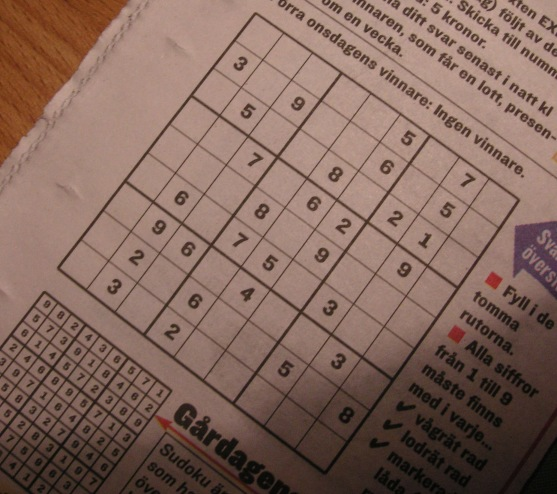
\includegraphics[width=10em]{sudoku81.jpg}
\end{figure}

If we want to extract the sudoku section of that image,

\begin{verbatim}
from scipy import ndimage
from PIL import Image

im = np.array(Image.open('sudoku81.JPG').convert('L'))
corners = [[257.4166, 14.9375], 
           [510.8489, 197.6145], 
           [59.30208, 269.65625], 
           [325.598958, 469.05729]]
corners = np.array(corners)
plt.plot(corners[:,0], corners[:,1], 'rd')
plt.imshow(im, cmap=plt.cm.Greys_r)
\end{verbatim}

Here picked corners of the image area are shown in red. 

Using the SVD calculation below,

I can obtain an $H$. Now I can warp the selection using my newly found $H$ and
retrieve the full-blown extracted image. 

\begin{verbatim}
def warpfcn(x):
    x = np.array([x[0],x[1],1])
    xt = np.dot(H,x)
    xt = xt/xt[2]
    return xt[0],xt[1]
im_g = ndimage.geometric_transform(im,warpfcn,(300,300))
\end{verbatim}

\begin{figure}[h]
  \centering
  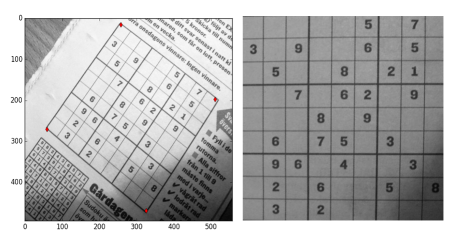
\includegraphics[width=22em]{out2.png}
\end{figure}


\section{Kalman Filters}


\section{Appendix: Code}

\subsection{Homography, SVD}

\begin{verbatim}
import scipy, numpy.linalg as lin
from scipy import ndimage

def H_from_points(fp,tp):
    if fp.shape != tp.shape:
        raise RuntimeError('number of points do not match')
        
    m = np.mean(fp[:2], axis=1)
    maxstd = np.max(np.std(fp[:2], axis=1)) + 1e-9
    C1 = np.diag([1/maxstd, 1/maxstd, 1]) 
    C1[0][2] = -m[0]/maxstd
    C1[1][2] = -m[1]/maxstd
    fp = np.dot(C1,fp)
    
    m = np.mean(tp[:2], axis=1)
    maxstd = np.max(np.std(tp[:2], axis=1)) + 1e-9
    C2 = np.diag([1/maxstd, 1/maxstd, 1])
    C2[0][2] = -m[0]/maxstd
    C2[1][2] = -m[1]/maxstd
    tp = np.dot(C2,tp)
    
    nbr_correspondences = fp.shape[1]
    A = np.zeros((2*nbr_correspondences,9))
    for i in range(nbr_correspondences):        
        A[2*i] = [-fp[0][i],-fp[1][i],-1,0,0,0,
                    tp[0][i]*fp[0][i],tp[0][i]*fp[1][i],tp[0][i]]
        A[2*i+1] = [0,0,0,-fp[0][i],-fp[1][i],-1,
                    tp[1][i]*fp[0][i],tp[1][i]*fp[1][i],tp[1][i]]
    
    U,S,V = lin.svd(A)
    H = V[8].reshape((3,3))    
    
    H = np.dot(lin.inv(C2),np.dot(H,C1))
    
    # normalize and return
    return H / H[2,2]

fp = [ [p[1],p[0],1] for p in corners]
fp = np.array(fp).T
tp = np.array([[0,0,1],[0,300,1],[300,0,1],[300,300,1]]).T
H = H_from_points(tp,fp)
\end{verbatim}


\bibliographystyle{unsrt}  

\begin{thebibliography}{1}

\bibitem{solem}
Solem, E. \emph{Programming Computer Vision with Python}, 2012

\bibitem{strang}
Strang, \emph{Too Much Calculus}, \url{http://web.mit.edu/18.06/www/Essays/too-much-calculus.pdf}

\end{thebibliography}

\end{document}
